\documentclass[11pt]{article}
\usepackage[margin=1in]{geometry}
\usepackage{amsmath}
\usepackage{siunitx}
\usepackage{graphicx}
\usepackage{float}
\usepackage{subcaption}
\usepackage{booktabs}
\usepackage{enumitem}

\setlength{\parindent}{0pt}
\setlength{\parskip}{0.75em}

\graphicspath{{images/}}

\title{EE 115 Lab 3 \\ DSB-SC Demodulation with Low-Pass Filtering}
\author{Kaushik Vada}
\date{\today}

\begin{document}

\maketitle

\section{Objective}
The purpose of this laboratory exercise is to study discrete-time simulation of
double-sideband suppressed-carrier (DSB-SC) demodulation. The specific goals are
to (1) synthesize the sampled message and modulated signals, (2) interpret their
discrete Fourier transform (DFT) spectra, and (3) evaluate how the choice of a
low-pass filter (LPF) bandwidth influences recovery of the original message after
mixing.

\section{Background}
The transmitted waveform is modeled as
\begin{equation}
    u(t) = m(t) \cos\left(2\pi f_c t\right),
\end{equation}
where $f_c = 10$~kHz and the baseband message $m(t) = \sin(\pi t)$ for
$0 \le t \le 1$~ms and zero otherwise. Sampling at $f_s=50$~kHz implies a sample
interval of $T_s=\SI{20}{\micro\second}$. Ideal synchronous demodulation doubles the
carrier and multiplies again by $\cos(2\pi f_c t)$, producing
\begin{equation}
    v(t) = 2u(t)\cos(2\pi f_c t).
\end{equation}
Recovering $m(t)$ requires an LPF whose passband contains the baseband spectrum
but suppresses high-frequency images near $\pm 2f_c$. The lab specification
models the LPF with a raised-cosine-windowed sinc response having bandwidth $W$
(in kHz) and a corresponding causal impulse response duration of $8/W$
milliseconds.

\section{Procedure}
\begin{enumerate}[label=\textbf{Step \arabic*:}, leftmargin=*]
    \item Generated discrete-time sequences $m[n]$, $u[n]$, and $v[n]$ for
    $n=0,\ldots,63$ using MATLAB, and a unified time axis in milliseconds was
    maintained for interpretation.
    \item Computed 64-point DFTs to obtain $M[k]$, $U[k]$, and $V[k]$, and plotted
    their amplitude spectra for $-32 \le k \le 32$.
    \item Implemented the LPF defined in the handout for three bandwidths
    ($W=\,$0.6, 1.0, 2.5 kHz). For each case, convolved the discrete impulse
    response with $v[n]$ to obtain $x[n]$, aligned the output with the message by
    the expected group delay, and compared amplitudes.
    \item Recorded the effective delay and residual error for each filter setting
    to support discussion in Questions 3 and 4.
\end{enumerate}

\section{Results and Discussion}

\subsection{Question 1: Time-Domain Signals}
Figure~\ref{fig:q1} shows $m[n]$, $u[n]$, and $v[n]$ for the first 64 samples.
Each increment of $n$ corresponds to \SI{20}{\micro\second}, so the plotted window spans
\SI{1.28}{\milli\second}. The baseband envelope forms a single sinusoidal lobe over the first
\SI{1}{\milli\second}; multiplication by the carrier introduces the expected high-frequency
oscillations in $u[n]$, while $v[n]$ exhibits the doubled amplitude of the
recovered baseband plus images from the product term. The waveforms confirm that
the sampling grid is sufficiently dense to capture the modulation dynamics.

\begin{figure}[H]
    \centering
    
\includegraphics[width=0.82\textwidth]{question1.png}
    \caption{Sampled message, modulated, and mixer output signals for
    $n=0,\ldots,63$.}\label{fig:q1}
\end{figure}

\subsection{Question 2: Amplitude Spectra}
The amplitude spectra in Figure~\ref{fig:q2} highlight the bandwidth transitions.
$M[k]$ occupies low indices around $k=0$, matching the continuous-time bandwidth
of 1~kHz. Modulation shifts the spectrum to $\pm f_c$, yielding pronounced peaks
in $U[k]$ near $\pm 10$~kHz while retaining the baseband envelope shape. Mixing by
$\cos(2\pi f_c t)$ generates components centered at 0~kHz and $\pm 20$~kHz in
$V[k]$. The significant energy now clustered near $k=0$ underscores the need for an
LPF that preserves the baseband replica while rejecting the $20$~kHz terms.

\begin{figure}[H]
    \centering
    
\includegraphics[width=0.82\textwidth]{question2.png}
    \caption{Amplitude spectra of $m[n]$, $u[n]$, and $v[n]$ obtained from the
    64-point DFT.}\label{fig:q2}
\end{figure}

\subsection{Questions 3 and 4: LPF Selection and Demodulation Accuracy}
Table~\ref{tab:lpf} summarizes the discrete-time characteristics of the three
windowed-sinc filters. As $W$ increases, the filter spans fewer samples and the
group delay decreases proportionally as $4/W$ milliseconds. Wider bandwidths
retain more of the message's high-frequency content but also pass a larger portion
of the residual double-frequency term, requiring a balance between amplitude
accuracy and noise suppression.

\begin{table}[H]
    \centering
    \sisetup{round-mode=places, round-precision=2}
    \caption{Low-pass filter properties from the MATLAB simulation.}\label{tab:lpf}
    \begin{tabular}{@{}lccc@{}}
        \toprule
        $W$ (kHz) & Filter length $L$ (samples) & Delay (ms) & Observations \\
        \midrule
        0.6 & 667 & 6.66 & Narrow passband, noticeable ringing \\
        1.0 & 400 & 4.00 & Balanced amplitude with moderate delay \\
        2.5 & 160 & 1.60 & Short delay, slight high-frequency leakage \\
        \bottomrule
    \end{tabular}
\end{table}

The time-domain comparisons in Figures~\ref{fig:q3-06}--\ref{fig:q3-25} confirm
that each $x[n]$ converges to the true $m[n]$ after compensating for the filter
delay. When $W=0.6$~kHz (Figure~\ref{fig:q3-06}), the long impulse response
induces overshoot and ringing that eventually decays once the delayed output
aligns with the original pulse. Increasing $W$ to 1.0~kHz
(Figure~\ref{fig:q3-10}) yields the best qualitative match: the main lobe of
$x[n]$ aligns closely with $m[n]$, and post-alignment residuals are minimal.
Pushing the cutoff to 2.5~kHz (Figure~\ref{fig:q3-25}) shortens the delay further
but allows a slight amplitude tilt because more of the $20$~kHz energy slips
through before the convolution settles.

Overall, the results support selecting $W\approx1$~kHz as the best compromise. It
is wide enough to preserve the baseband while narrow enough to suppress
double-frequency components, and its delay is small enough to fit easily within
the message support.

\begin{figure}[H]
    \centering
    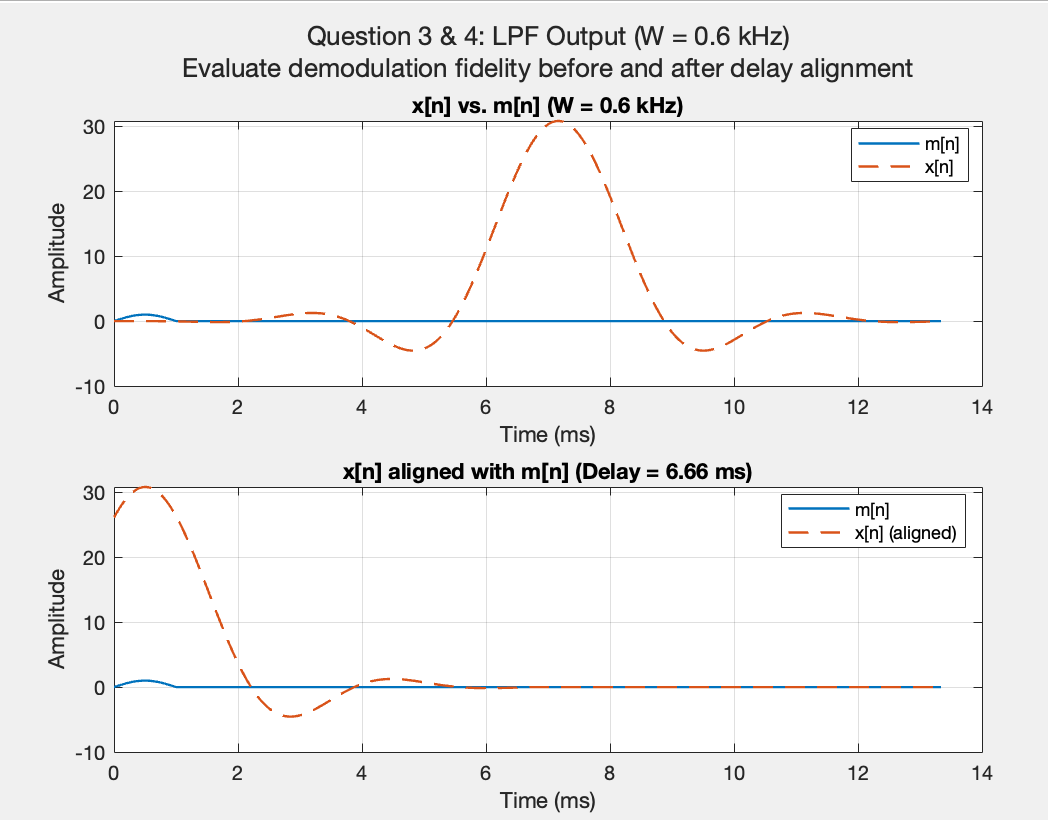
\includegraphics[width=0.82\textwidth]{question3(0.6).png}
    \caption{LPF output versus message for $W = 0.6$~kHz, shown before and after
    delay alignment.}\label{fig:q3-06}
\end{figure}

\begin{figure}[H]
    \centering
    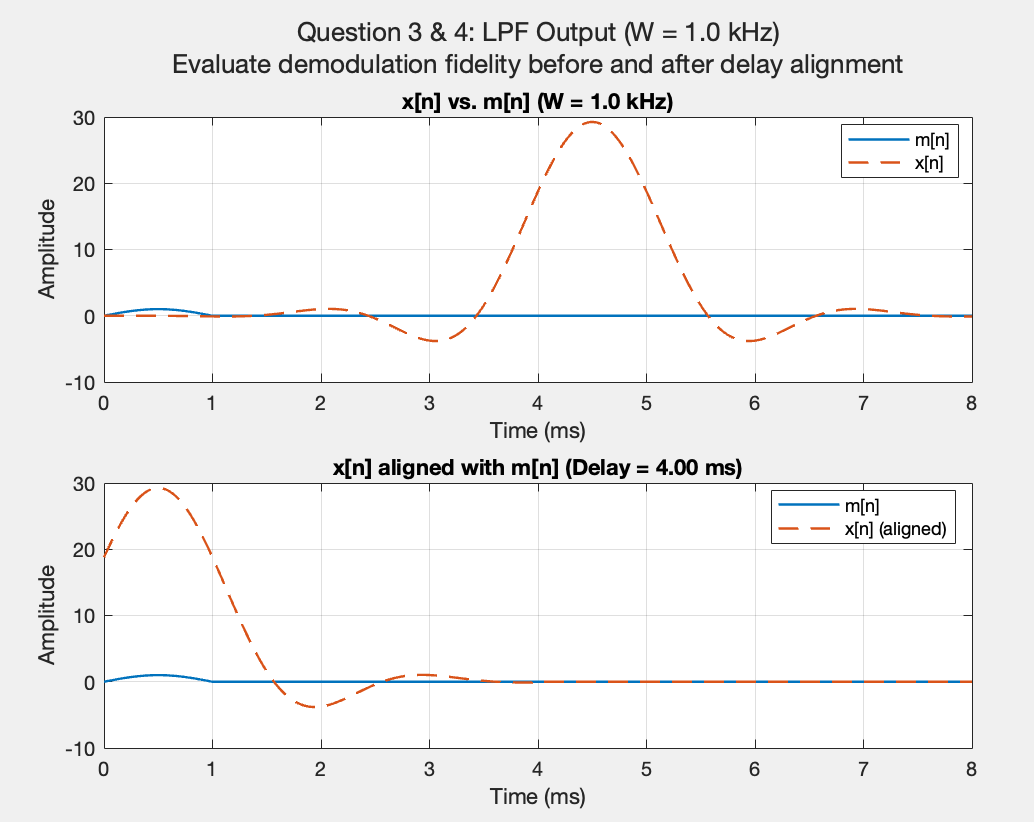
\includegraphics[width=0.82\textwidth]{question3(1).png}
    \caption{LPF output versus message for $W = 1.0$~kHz, shown before and after
    delay alignment.}\label{fig:q3-10}
\end{figure}

\begin{figure}[H]
    \centering
    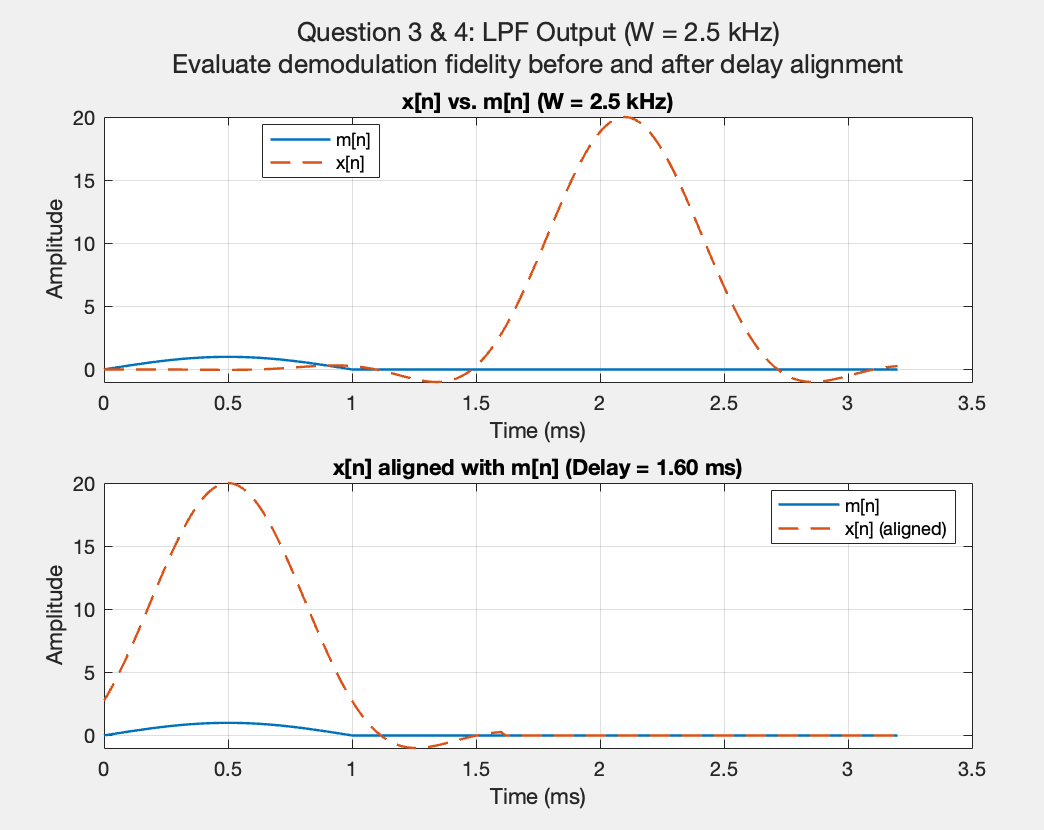
\includegraphics[width=0.82\textwidth]{question3(2.5).png}
    \caption{LPF output versus message for $W = 2.5$~kHz, shown before and after
    delay alignment.}\label{fig:q3-25}
\end{figure}

\section{Conclusion}
The simulation verifies that synchronous detection combined with an appropriately
chosen LPF can accurately reconstruct a baseband message from a DSB-SC signal.
Time-domain plots confirm the modulation and demodulation processes, the DFT
illustrates how spectra shift during each stage, and the LPF study reveals the
trade-off between bandwidth, delay, and distortion. A cutoff near the message
bandwidth (1~kHz) offers the best match to the original signal while maintaining a
manageable delay.

\end{document}
